\documentclass{beamer}

\mode<presentation> {
%    \usetheme{Madrid}
%    \usetheme{Warsaw}
%    \usetheme{Berlin}
    \usetheme{CambridgeUS}
}

%\usepackage{cite}
\usepackage{amsmath}
\usepackage{amsfonts}
\usepackage{amssymb}
\usepackage{bm}
\usepackage{subcaption}
\usepackage{caption}
\usepackage{xspace}
\usepackage{afterpage}
%\usepackage{color}
%\usepackage[dvipsnames,table,xcdraw]{xcolor}
\usepackage{stmaryrd}
\usepackage{textcomp}
\usepackage{natbib}
\usepackage{multicol}
\usepackage{xcolor}
%\usepackage[mathb]{mathabx}
\usepackage[absolute,overlay]{textpos}

% hyperref must be last
\usepackage{hyperref}
\hypersetup{
%    backref=true,
%    colorlinks=true,
%    linkcolor=blue,
%    citecolor=blue,
%    urlcolor=blue
}
\setbeamercolor{frametitle}{bg=gray!15}
\setbeamertemplate{caption}[numbered]
\setbeamercolor{block body}{bg=gray!20!white}


% Update footline template to have a 1:2:1 ratio in the boxes
\setbeamertemplate{footline}{%
    \leavevmode%
    \hbox{%
        \begin{beamercolorbox}[wd=.25\paperwidth,ht=2.5ex,dp=1.125ex, left]{author in head/foot}%
            \usebeamerfont{author in head/foot}\hspace*{3ex}\insertshortauthor
        \end{beamercolorbox}%
        \begin{beamercolorbox}[wd=.5\paperwidth,ht=2.5ex,dp=1.125ex,center]{title in head/foot}%
            \usebeamerfont{title in head/foot}\insertshorttitle
        \end{beamercolorbox}%
        \begin{beamercolorbox}[wd=.25\paperwidth,ht=2.5ex,dp=1.125ex,right]{title in head/foot}%
            \usebeamerfont{date in head/foot}\insertshortdate{}
            \insertframenumber{} / \inserttotalframenumber\hspace*{4ex} 
        \end{beamercolorbox}
    }%
    \vskip0pt%
}

% input file that defines new command

\newcommand{\fnc}[1]{\ensuremath{\mathcal{#1}}}
\newcommand{\vecfnc}[1]{\ensuremath{\boldsymbol{\mathcal{#1}}}} % vector function

% matrices are often math sans serif type
\newcommand{\mat}[1]{\ensuremath{\mathsf{#1}}}

\newcommand{\mr}[1]{\mathrm{#1}}
\newcommand{\diff}[0]{\mr{d}}
\newcommand{\Tr}[0]{^\mr{T}}

% SBP operator matrices
\renewcommand{\H}[0]{\mat{H}}
\newcommand{\Hk}[0]{\H_{\kappa}}
\newcommand{\D}[0]{\mat{D}}
\newcommand{\Dx}[0]{\mat{D}_{x}}
\newcommand{\Dy}[0]{\mat{D}_{y}}
\newcommand{\Dz}[0]{\mat{D}_{z}}
\newcommand{\Skew}[0]{\mat{S}}
\newcommand{\Sx}[0]{\Skew_{x}}
\newcommand{\Sy}[0]{\Skew_{y}}
\newcommand{\Sz}[0]{\Skew_{z}}
\newcommand{\Q}[0]{\mat{Q}}
\newcommand{\Qx}[0]{\mat{Q}_{x}}
\newcommand{\Qy}[0]{\mat{Q}_{y}}
\newcommand{\Qz}[0]{\mat{Q}_{z}}
\newcommand{\E}[0]{\mat{E}}
\newcommand{\Ex}[0]{\mat{E}_{x}}
\newcommand{\Ey}[0]{\mat{E}_{y}}
\newcommand{\Ez}[0]{\mat{E}_{z}}
\newcommand{\R}[0]{\mat{R}}
\newcommand{\B}[0]{\mat{B}}
\newcommand{\Bg}[0]{\mat{B}_{\gamma}}
\newcommand{\Gk}[0]{\mat{F}_{\kappa}}
\newcommand{\Gn}[0]{\mat{F}_{\nu}}
\newcommand{\Cgk}[0]{\mat{C}_{\gamma\kappa}}
\newcommand{\Cgn}[0]{\mat{C}_{\gamma\nu}}
%\newcommand{\Lxk}[0]{\bm{l}_{x,\kappa}^{\gamma}}
%\newcommand{\Lyk}[0]{\bm{l}_{y,\kappa}^{\gamma}}
%\newcommand{\Lxn}[0]{\bm{l}_{x,\nu}^{\gamma}}
%\newcommand{\Lyn}[0]{\bm{l}_{y,\nu}^{\gamma}}
\newcommand{\Sig}[0]{\mat{\Sigma}}
\newcommand{\Lam}[0]{\mat{\Lambda}}
\newcommand{\Lamxx}[0]{\Lam_{xx}}
\newcommand{\Lamxy}[0]{\Lam_{xy}}
\newcommand{\Lamyx}[0]{\Lam_{yx}}
\newcommand{\Lamyy}[0]{\Lam_{yy}}

\newcommand{\fpk}{\fnc{P}_{k}}
\newcommand{\fpm}{\fnc{P}_{m}}
\newcommand{\pk}{\bm{p}_{k}}
\newcommand{\pM}{\bm{p}_{m}}
\newcommand{\dxfpk}{\frac{\partial\fnc{P}_{k}}{\partial x}}
\newcommand{\dxpk}{\bm{p}_{k}'}
\newcommand{\nmin}[1]{N^{*}_{#1}}
\newcommand{\nk}[0]{n_{\kappa}}

\newcommand{\poly}[1]{\mathbb{P}_{#1}}
\newcommand{\J}[0]{|\mat{J}|^{-1}}
\newcommand{\N}[0]{|\mat{N}^*|}
\newcommand{\Nx}[0]{\mat{N}_x}
\newcommand{\Ny}[0]{\mat{N}_y}
\newcommand{\Nxg}[0]{\mat{N}_{x,\gamma}}
\newcommand{\Nyg}[0]{\mat{N}_{y,\gamma}}
\newcommand{\Rg}[0]{\mat{R}_{\gamma}}
\newcommand{\Rgk}[0]{\mat{R}_{\gamma\kappa}}
\newcommand{\Rgn}[0]{\mat{R}_{\gamma\nu}}
\newcommand{\Dg}[0]{\mat{D}_{\gamma}}
\newcommand{\Dgk}[0]{\mat{D}_{\gamma\kappa}}
\newcommand{\Dgn}[0]{\mat{D}_{\gamma\nu}}
\newcommand{\Ukp}[0]{\bm{u}_\kappa}
\newcommand{\Vkp}[0]{\bm{v}_\kappa}
\newcommand{\Unu}[0]{\bm{u}_\nu}
\newcommand{\Vnu}[0]{\bm{v}_\nu}
\newcommand{\Wkp}[0]{\bm{w}_\kappa}
\newcommand{\Wnu}[0]{\bm{w}_\nu}
\newcommand{\Ugam}[0]{\bm{u}_\gamma}
\newcommand{\W}[0]{\bm{w}}
%\newcommand{\Gk}{\Gamma_\kappa}
\newcommand{\SumAll}{\sum_{\Omega_\kappa \in \fnc{T}_h}}
\newcommand{\M}[0]{\mat{M}}
\newcommand{\Mk}[0]{\mat{M}_{\kappa}}

\newcommand{\Uh}{\bm{u}_{h}}
\newcommand{\Vh}{\bm{v}_{h}}
\newcommand{\Ug}{\bm{u}_{\gamma}}
\newcommand{\Vg}{\bm{v}_{\gamma}}
\newcommand{\Siggk}[1]{\Sig_{\gamma\kappa}^{(#1)}}
\newcommand{\Siggn}[1]{\Sig_{\gamma\nu}   ^{(#1)}}
\newcommand{\Siggam}[1]{\Sig_{\gamma}^{(#1)}}
\newcommand{\phnt}[1]{\phantom{#1}}

\newcommand{\LL}{\llbracket}
\newcommand{\RR}{\rrbracket}

% optimization commands
\newcommand{\Lag}[0]{\fnc{L}}
\newcommand{\optmin}{\ensuremath{\text{minimize}}}
\newcommand{\wrt}{\ensuremath{\text{with respect to}}}
\newcommand{\st}[0]{\ensuremath{\text{s.t.}}}
%\newcommand{\W}[0]{\mat{W}} % Hessian
\newcommand{\A}[0]{\mat{A}} % Jacobian
%\newcommand{\K}[0]{\mat{K}} % KKT matrix
\newcommand{\Hess}[0]{\mat{H}} % upper Hessenberg
\newcommand{\I}[0]{\mat{I}} % identity

% common math operators
\DeclareMathOperator{\spn}{span}
\DeclareMathOperator{\range}{range}
\DeclareMathOperator{\mydiag}{diag}
\newcommand{\argmin}[0]{\ensuremath{\operatornamewithlimits{argmin}}}
\newcommand{\sgn}[0]{\operatorname{sgn}}
\newcommand{\nullsp}[0]{\operatorname{null}}

% environments for definitions, therorems, etc 
%\newtheorem{definition}{Definition}
%\newtheorem{proposition}{Proposition}
%\newtheorem{corollary}{Corollary}
%\newtheorem{lemma}{Lemma}
%\newtheorem{remark}{Remark}
\newtheorem{assumption}{Assumption}
\newtheorem{thrm}{Theorem}

% command latin phrases and other short-forms
\newcommand{\etal}[0]{{\em et~al.\@}\xspace}
\newcommand{\eg}[0]{{e.g.\@}\xspace}
\newcommand{\ie}[0]{{i.e.\@}\xspace}
\newcommand{\etc}[0]{{etc.\@}\xspace}
\newcommand{\viz}[0]{{viz.\@}\xspace}
\newcommand{\resp}[0]{{resp.\@}\xspace}

\newcommand{\highlight}[1]{%
    \colorbox{red!50}{$\displaystyle#1$}
}

\newenvironment<>{varblock}[2][.9\textwidth]{%
    \setlength{\textwidth}{#1}
    \begin{actionenv}#3%
        \def\insertblocktitle{#2}%
        \par%
        \usebeamertemplate{block begin}
    }
        {\par%
        \usebeamertemplate{block end}%
    \end{actionenv}
}





\title[Interior Penalties for SBP Discretizations of 2nd PDEs]{Interior Penalties for Summation-by-Parts Discretizations of Linear Second-Order Differential Equations}
\author[Yan \textit{et al}]{Jianfeng Yan, Jared Crean, and Jason E. Hicken}
\institute[]{\normalsize Dept. of Mechanical, Aerospace, Nuclear Enginnering \\ Rensselaer Polytechnic Institute \\
    \vskip 5mm
2017 Aviation, Denver, CO}
\date[]
{ AIAA-2017-4495}


\AtBeginSection[]{
    \begin{frame}<beamer>
         \tableofcontents[currentsection,hideallsubsections]
%         \tableofcontents[currentsection,hideothersubsections]
    \end{frame}
}
\setbeamerfont{section in toc}{size=\normalsize}
\setbeamerfont{subsection in toc}{size=\small}

%
% Start the document
%
\begin{document}
\begin{frame}
    \titlepage
\end{frame}

\begin{frame}{SBP operators}
    Summation-by-parts (SBP) operators are high-order finite difference methods that:
    \begin{itemize}
        \item mimic integration by parts
        \item have compact stencil support
        \item do not depend on exact integration
        \item have no explicit basis and test functions in general
        \item facilitate construction of entropy-stable discretizations of Euler and Navier-Stokes equations
    \end{itemize}
\end{frame}

\begin{frame}
    Classical SBP operators:
    \begin{itemize}
        \item based on tensor products of 1D operators;
        \item limited to structured grids.
    \end{itemize}
    Multidimensional SBP operators:
    \begin{itemize}
        \item recently introduced by Hicken, Del Rey Fernandez and Zingg;
        \item applies to arbitrary bounded domains.
    \end{itemize}
    
    \vskip 10mm
    \centering
    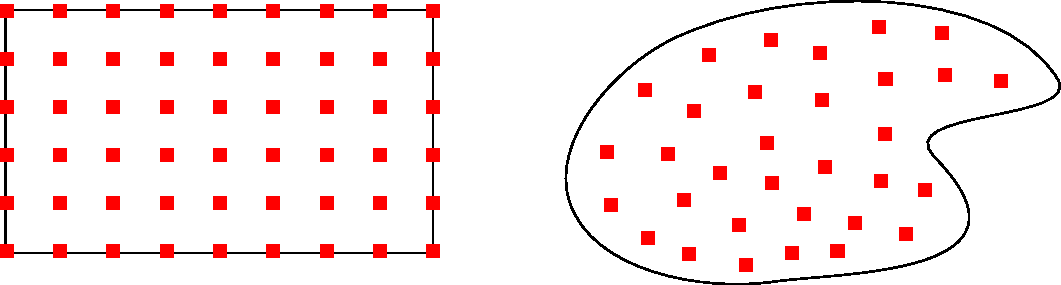
\includegraphics[width=0.75\textwidth]{./figures/generalize_tensor.pdf}
\end{frame}

\begin{frame}{Interior penalties for 2nd derivatives}
    Since the solution is "$C^{-1}$" continuous, simultaneous 
    approximation terms (SATs) are necessary to couple elements weakly, and 
    \begin{itemize}
        \item are referred as interior penalties in the FE community
        \item stabilize the discretization the penalties should be \\ neither too large nor too small in magnitude (Arnold 2002)
        \item obtain adjoint consistency \\
        optimal convergence rates for solution and functionals
        
    \end{itemize}
    \vskip 5mm
    The purpose of this work is to address SATs for multidimensional SBP.
\end{frame}

\begin{frame}{Outline}
    \tableofcontents[hideallsubsections]
\end{frame}

\section{Model PDE and discretizations}

\begin{frame}
    \begin{definition}{}
        \textbf{SBP operators:} Consider an element $\kappa \subset \mathbb{R}^2$. The matrix $D_x$ is a degree $p$ SBP approximation to the first derivative $\frac{\partial}{\partial x}$ if 
        \begin{itemize}
            \item $\forall \fnc{P} \in \poly{p}(\Omega_{\kappa})$, $\Dx\pk = \partial \fnc{P}/\partial x |_{\kappa}$;
            \item $\Dx = \H^{-1}\Qx$, where $\H$ is symmetric positive-definite;
            \item $\Qx = \Sx + \frac{1}{2}\Ex$, where $\Sx^T=-\Sx$, $\Ex^T=\Ex$, and
            $\Ex$ satisfies
            \begin{equation*}
            \bm{p}^T\Ex\bm{q} =\displaystyle\oint_{\partial{\kappa}} \fnc{P} \fnc{Q} n_{x}
            \mr{d}\Gamma,
            \qquad\forall\; \fnc{P}, \fnc{Q} \in \poly{r}({\kappa}).
            \end{equation*}
        \end{itemize}
    \end{definition}

    \vskip 3mm
    \begin{equation*}
    \begin{aligned}
        &\int \fnc{P}\frac{\partial \fnc{Q}}{\partial x}\diff \Omega &&= &&&\int  \fnc{P} \fnc{Q} n_{x}
        \diff\Gamma &&&&- &&&&& \int \fnc{Q}\frac{\partial \fnc{P}}{\partial x}\diff \Omega \\
        &\bm{p}^T \H \Dx \bm{q} && = &&&\bm{p}^T\Ex\bm{q} &&&&- &&&&&\bm{q}^T \H \Dx \bm{p}
    \end{aligned}
    \end{equation*}
\end{frame}

\begin{frame} {Face operators}
    We also introduce $\Rgk \in \mathbb{R}^{n_\gamma \times n_\kappa}$, a degree $r \le p$ interpolation/extrapolation operator which satisfies
    \begin{equation*}
    \left(\Rgk \pk\right)_{j} = 
    \sum_{i=1}^{\nk} (\Rgk)_{ji} \fnc{P}(x_{i},y_{i}) 
    = \fnc{P}(x_{j},y_{j}),
    \qquad\forall j=1,2,\ldots,n_{\gamma}.
    \end{equation*}
    then we can find SBP operators with \\ \vskip 3mm
%    \begin{equation*}
$\qquad
    \Ex = \sum_{\gamma \subset \partial \kappa} \Rgk^{T} \Nxg \Bg \Rgk,
$\\ \vskip 3mm
%    \end{equation*}
    Thus \\ \vskip 2mm
%    \begin{equation*}
$\qquad
    \bm{p}^T \Ex \bm{q} = \sum_{\gamma \in \partial\kappa} \bm{p}^T \Rgk^T\Nxg\B_{\gamma}\Rgk\bm{q} = \int_{\partial\kappa}\fnc{P}\fnc{Q} n_x\diff \Gamma
$
%    \end{equation*}
    
    \begin{textblock}{5.55}(9.0,8.0)
        \includegraphics[width=1.1\textwidth]{./figures/element_illustration.png}
    \end{textblock}
    
\end{frame}

\begin{frame}{The model PDE}
    We consider the following linear parabolic PDE:
    \begin{equation*}\label{eq:parabolic}
    \begin{aligned}
    \frac{\partial \fnc{U}}{\partial{t}}- \nabla\cdot\left( \Lambda \nabla \fnc{U} \right) &= \fnc{F},\quad &&\text{in} \quad\Omega, \\
    \fnc{U}(0,x,y)&=\fnc{U}_{0}(x,y), \quad &&\text{in} \quad\Omega, \\
    \fnc{U}(t,x,y) &= \fnc{U}_\fnc{D}(t,x,y) &&\text{on} \quad\Gamma^\fnc{D}, \\
    \hat{\bm{n}} \cdot \left( \Lambda \nabla \fnc{U}(t,x,y)\right) &= \fnc{U}_\fnc{N}(t,x,y)
    &&\text{on} \quad \Gamma^\fnc{N}. \\
    \end{aligned}
    \end{equation*}
    where
    \begin{equation*}
    \Lambda = \begin{bmatrix}
    \lambda_{xx} & \lambda_{xy} \\ \lambda_{yx} & \lambda_{yy}
    \end{bmatrix}
    \end{equation*}
    is symmetric positive definite.
\end{frame}

\begin{frame}{Strong-form discretization}
    \begin{equation*}
    {\color{red}\frac{\partial \fnc{U}}{\partial{t}}}- {\color{blue}\nabla\cdot\left( \Lambda \nabla \fnc{U} \right)} = {\color{purple}\fnc{F}},\quad \text{in} \quad\Omega
    \end{equation*}
    \vskip 5mm
The strong-form SBP-SAT discretization on element $\kappa$ is given by
\begin{equation*}
{\color{red}\frac{\diff \bm{u}_{\kappa}}{\diff t}} = {\color{blue}\D_\kappa\bm{u}_{\kappa}} + {\color{purple}\bm{f}_\kappa },
\end{equation*}
where 
\begin{equation*}
\D_\kappa = \left\{ \begin{bmatrix} \Dx & \Dy \end{bmatrix}
\begin{bmatrix} \Lamxx & \Lamxy \\ \Lamyx & \Lamyy \end{bmatrix}
\begin{bmatrix} \Dx \\ \Dy \end{bmatrix} \right\}_{\kappa},
\end{equation*}
\end{frame}

\begin{frame}{Strong-form discretization}
    \begin{equation*}
    {\color{red}\frac{\partial \fnc{U}}{\partial{t}}}- {\color{blue}\nabla\cdot\left( \Lambda \nabla \fnc{U} \right)} = {\color{purple}\fnc{F}},\quad \text{in} \quad\Omega
    \end{equation*}
    \vskip 5mm
    The strong-form SBP-SAT discretization on element $\kappa$ is given by
    \begin{equation*}
    {\color{red}\frac{\diff \bm{u}_{\kappa}}{\diff t}} = {\color{blue}\D_\kappa\bm{u}_{\kappa}} + {\color{purple}\bm{f}_\kappa }
    -\Hk^{-1}\bm{s}_{\kappa}^{\fnc{I}}\left(\bm{u}_{h}\right) 
    -\Hk^{-1}\bm{s}_{\kappa}^{\fnc{B}}\left(\bm{u}_{h}, \bm{u}_\fnc{D}, \bm{u}_\fnc{N}\right),
    \end{equation*}
    
    \begin{itemize}
        \item interior penalty to couple elements;
        \item boundary penalty to enforce BCs.
    \end{itemize}
\end{frame}


\begin{frame}{Strong form discretization}
    The interior penalty 
    \vskip -3mm
    \begin{equation*}
    \bm{s}_{\kappa}^{\fnc{I}}\left(\bm{u}_{h}\right)
    = \sum_{\gamma \subset \Gamma_\kappa^\fnc{I}}
    \begin{bmatrix} \Rgk^T & \Dgk^T \end{bmatrix}
    \setlength{\arraycolsep}{7pt}
    {\color{blue}\begin{bmatrix} \Siggk{1} & \Siggk{3} \\ \Siggk{2} & \Siggk{4} \end{bmatrix}}
    {\color{red}\begin{bmatrix} \Rgk\Ukp - \Rgn\Unu \\ \Dgk\Ukp + \Dgn\Unu \end{bmatrix} }
    \end{equation*}
    is analogous to
    \vskip -3mm
    \begin{equation*}
    \int_{\gamma} 
    \begin{bmatrix} \llbracket\fnc{V} \rrbracket \\ \llbracket \bm{n}\cdot \nabla\fnc{V}\rrbracket \end{bmatrix}^T
    {\color{blue}\begin{bmatrix}
        \sigma_1 && \sigma_2 \\ \sigma_3 && \sigma_4
        \end{bmatrix}}
    {\color{red}\begin{bmatrix}
        \llbracket\fnc{U} \rrbracket \\ 
        \llbracket \bm{n}\cdot \nabla\fnc{U}\rrbracket
        \end{bmatrix}} \diff \Gamma
    \end{equation*}
    \vskip 2mm
    Assumptions on penalty matrices:
    \begin{itemize}
        \item $\Sig_{\gamma\kappa}^{(i)} \in \mathbb{R}^{n_\gamma\times n_\gamma}$, are \textbf{dense};
        \item \textbf{symmetric}, $\Sig_{\gamma\kappa}^{(i)} = (\Sig_{\gamma\kappa}^{(i)})^T$;
        \item $\Sig_{\gamma\kappa}^{(i)} \ne \Sig_{\gamma\nu}^{(i)}$ in general.
    \end{itemize}
\end{frame}

\begin{frame}
    The boundary penalty is defined similarly
    \begin{equation*}
    \begin{aligned}
    \bm{s}_{\kappa}^{\fnc{B}}\left(\bm{u}_{h}, \bm{u}_\fnc{D}, \bm{u}_\fnc{N}\right)
    =& \sum_{\gamma \subset \Gamma_\kappa^{\fnc{D}}}
    \begin{bmatrix} \Rgk^T & \Dgk^T \end{bmatrix}
    \begin{bmatrix} \phnt{-}\Sig_{\gamma}^{\fnc{D}} \\ -\Bg \end{bmatrix}
    (\Rgk \Ukp -\bm{u}_{\gamma {\fnc{D}}}) \\
    +& \sum_{\gamma \subset \Gamma_\kappa^{\fnc{N}}} \Rgk^{T}\B_{\gamma} (\Dgk \Ukp - \bm{u}_{\gamma {\fnc{N}}})
    \end{aligned}
    \end{equation*}
\end{frame}

\section{Adjoint analysis}

\begin{frame}{Adjoint consistency}
    Adjoint consistency
    \begin{itemize}
        \item discrete adjoint equation consistent to continuous adjoint equation;
        \item $O(h^{p+1})$ in solution in terms of $L^2$-norm, and $O(h^{2p})$ in functional;
        \item smooth adjoint solutions.
    \end{itemize}
\end{frame}
\begin{frame}{Adjoint equations}
    An adjoint is defined by the primal PDE and a particular functional of interest. We consider the linear functional
    \begin{equation*}
    \fnc{J}(\fnc{U}) = {\color{red}\int_{\Omega} \fnc{G} \fnc{U} \, \diff \Omega}
    +  {\color{blue}\int_{\Gamma^\fnc{N}} \fnc{V}_\fnc{N} \fnc{U} \, \diff\Gamma }
    -  {\color{purple}\int_{\Gamma^\fnc{D}} \fnc{V}_\fnc{D} \hat{\bm{n}} \cdot \left(\Lambda \nabla \fnc{U} \right) \, \diff\Gamma} ,
    \end{equation*}
    and its SBP discretization
    \begin{equation*}
    \begin{aligned}
    J_h(\bm{u}_h) :=& {\color{red}\sum_{\kappa \in \fnc{T}_{h}}\bm{g}_{\kappa}^T\Hk\Ukp}
    + {\color{blue}\sum_{\gamma \subset \Gamma^{\fnc{N}}} \bm{v}_{\gamma \fnc{N}}^T\Bg\Rgk\Ukp}
    - {\color{purple}\sum_{\gamma \subset \Gamma^{\fnc{D}}} \bm{v}_{\gamma \fnc{D}}^T\Bg\Dgk\Ukp} \\
    +& \sum_{\gamma \subset \Gamma^{\fnc{D}}} \bm{v}_{\gamma \fnc{D}}^T\Sig_{\gamma}^{\fnc{D}} (\Rgk\Ukp - \bm{u}_{\gamma \fnc{D}})
    \end{aligned}
    \end{equation*}
\end{frame}
\begin{frame}{Adjoint equations}
    \Large
    $\frac{\delta L}{\delta u} = 0$ \normalsize gives adjoint equations.
    
    \vskip 2mm
    \begin{itemize}
        \item Continous adjoint equation:
        \begin{equation*}
        \begin{aligned}
        -&\nabla\cdot\left(\Lambda \nabla\fnc{V} \right) = \fnc{G},\quad &&\forall \; x \in \Omega, \\
        &\fnc{V} = \fnc{V}_\fnc{D}, \quad &&\forall \; x \in \Gamma^\fnc{D},  \\
        &\hat{\bm{n}} \cdot \left( \Lambda \nabla \fnc{V}\right) = \fnc{V}_\fnc{N},
        &&\forall \; x \in \Gamma^\fnc{N}.
        \end{aligned}
        \end{equation*}
        \item Discrete adjoint equation:
        \begin{equation*}\label{eq:adjoint_SBP}
        \D_{\kappa} \Vkp + \bm{g}_{\kappa}
        - \Hk^{-1} (\bm{s}_{\kappa}^{\fnc{I}})^{*}(\bm{v}_h)
        - \Hk^{-1} (\bm{s}_{\kappa}^{\fnc{B}})^{*}(\bm{v}_h,\bm{v}_\fnc{D},\bm{v}_\fnc{N})
        = \bm{0}.
        \end{equation*}
    \end{itemize}
\end{frame}

\begin{frame}{Adjoint equations}
    Interior penalty
    \footnotesize
    \begin{equation*} \label{ad_interface_sat}
    (\bm{s}_{\kappa}^{\fnc{I}})^{*}\left(\bm{v}_{h}\right)
    = \sum_{\gamma \subset \Gamma_\kappa^\fnc{I}}
    \begin{bmatrix} \Rgk^T & \Dgk^T \end{bmatrix}
    \setlength{\arraycolsep}{7pt}
    \setlength{\arraycolsep}{5pt}
    \begin{bmatrix}
    \phnt{-}\Siggk{1}       & -\Siggn{1}      & \Siggk{2} + \Bg & -\Siggn{2} \\
    \Siggk{3} - \Bg & \phnt{-}\Siggn{3}       & \phnt{-}\Siggk{4}       & \phnt{-}\Siggn{4}
    \end{bmatrix}
    \begin{bmatrix} \Rgk \Vkp \\ \Rgn \Vnu \\ \Dgk \Vkp \\ \Dgn \Vnu \end{bmatrix} 
    \end{equation*}
    \normalsize
    and the boundary penalty
    \footnotesize
    \begin{equation*}
    \begin{aligned}
    (\bm{s}_{\kappa}^{\fnc{B}})^{*}\left(\bm{v}_{h}, \bm{v}_\fnc{D}, \bm{v}_\fnc{N}\right)
    =& \sum_{\gamma \subset \Gamma_\kappa^{\fnc{D}}}
    \begin{bmatrix} \Rgk^T & \Dgk^T \end{bmatrix}
    \begin{bmatrix} \phnt{-}\Sig_{\gamma}^{\fnc{D}} \\ -\Bg \end{bmatrix}
    (\Rgk \Vkp - \bm{v}_{\gamma\fnc{D}}) \\
    +& \sum_{\gamma \subset \Gamma_\kappa^{\fnc{N}}} \Rgk^{T}\B_{\gamma} (\Dgk \Vkp - \bm{v}_{\gamma\fnc{N}}).
    \end{aligned}
    \end{equation*} 
\end{frame}

\begin{frame}{Adjoint consistency}
    The definition of adjoint consistency requires 
    \begin{equation*}
        (\bm{s}^{\fnc{I}})^{*} = (\bm{s}^{\fnc{B}})^{*} = \bm{0}
    \end{equation*}
    Conditions for adjoint consistency:
    \begin{block}{}
        \begin{equation*}
        \begin{aligned}
        \Siggk{1} &= \Siggn{1}, &\qquad  
        \Siggk{2} + \Siggn{2} &= -\B_{\gamma}, \\
        \Siggk{3} + \Siggn{3} &= \B_{\gamma}, &\qquad
        \Siggk{4} &= \Siggn{4}.
        \end{aligned}
        \end{equation*}
    \end{block}

\vskip 5mm
It is straightforward to show the above conditions also give a locally \textbf{conservative} discretization.

\end{frame}

\section{Energy analysis}
\subsection{Energy of PDE}
\begin{frame} {Energy of homogeneous problem}
    The solution of the homogeneous PDE, $\fnc{W}$, satisfies
    \begin{equation*}
    \frac{1}{2} \frac{\diff}{\diff t} \int_{\Omega} \fnc{W}^{2} \, \diff \Omega
    = - \int_{\Omega} \left(\nabla \fnc{W}\right) \cdot \Lambda \left(\nabla \fnc{W} \right) \, \diff \Omega
    \le 0.
    \end{equation*}
    We want the discrete energy to mimic this property.
\end{frame}
\subsection{Stability conditions}
\begin{frame} {Stability conditions}
    With the assumption
    \begin{equation*}
    \Siggk{3} - \Siggk{2} = \Bg,
    \end{equation*}
    we get
    \small
    \begin{equation*}
    \begin{aligned}
     &\sum_{\kappa\in \fnc{T}_h}\Ukp^T \Hk \frac{\diff \Ukp}{\diff t} = \\
    -& \sum_{\gamma \subset \Gamma^{\fnc{I}}}
    {\color{red}\begin{bmatrix} \Rgk \Ukp \\ \Rgn \Unu \\ \Gk \Ukp \\ \Gn \Unu
    \end{bmatrix}^{T}} 
    \setlength{\arraycolsep}{5pt}
    \begin{bmatrix} 
    \phnt{-}\Siggam{1} & -\Siggam{1} & \phnt{-}\Siggk{2} \Cgk & -\Siggn{2}\Cgn \\
    -\Siggam{1} & \phnt{-}\Siggam{1} & -\Siggk{2}\Cgk & \phnt{-}\Siggn{2}\Cgn \\
    \phnt{-}\Cgk^T\Siggk{2} & -\Cgk^{T}\Siggk{2} & \alpha_{\gamma \kappa}\Lam_{\kappa}^{*} &  \\
    -\Cgn^T\Siggn{2} & \phnt{-}\Cgn^{T}\Siggn{2} &  & \alpha_{\gamma \nu} \Lam_{\nu}^{*}   
    \end{bmatrix}
    \begin{bmatrix} \Rgk \Ukp \\ \Rgn \Unu \\ \Gk \Ukp \\ \Gn \Unu
    \end{bmatrix} \\
    -& \sum_{\gamma \subset \Gamma^{\fnc{I}}}
    \begin{bmatrix} \Dgk \Ukp \\ \Dgn \Unu \end{bmatrix}^T
    \begin{bmatrix} \Siggam{4} & \Siggam{4} \\ \Siggam{4} & \Siggam{4} \end{bmatrix}
    \begin{bmatrix} \Dgk \Ukp \\ \Dgn \Unu \end{bmatrix} \\
    -& \sum_{\gamma \subset \Gamma^{\fnc{D}}}
    \begin{bmatrix} \Rgk \Ukp \\ \Gk \Ukp \end{bmatrix}^{T}
    \setlength{\arraycolsep}{5pt}
    \begin{bmatrix} \phnt{-}\Sig_{\gamma}^{\fnc{D}} & -\Bg \Cgk \\
    -\Cgk^T \Bg & \alpha_{\gamma \kappa}\Lam_{\kappa}^{*} \end{bmatrix}
    \begin{bmatrix} \Rgk \Ukp \\ \Gk \Ukp \end{bmatrix},
    \end{aligned}
    \end{equation*}
    \footnotesize
    \begin{textblock}{5.55}(10.5,4.5)
        \textblockcolor{gray!30}
%        \centering
        $\int 
        {\color{red}\begin{bmatrix}
            u^+ \\ u^- \\ (\Lambda\nabla u)^+ \\ (\Lambda\nabla u)^-
        \end{bmatrix}^T}
        K\begin{bmatrix}
            u^+ \\ u^- \\ (\Lambda\nabla u)^+ \\ (\Lambda\nabla u)^-
        \end{bmatrix} 
        \diff \Gamma $
    \end{textblock}

\end{frame}


%\begin{frame}{Stability conditions}
%    where
%    \begin{equation*}
%    \alpha_{\gamma\kappa} \ge 0 \qquad and \qquad \sum_{\gamma\subset \Gamma_{\kappa}} \alpha_{\gamma\kappa} = 1,
%    \end{equation*}
%    \begin{alignat*}{2}
%    \Gk &= \left\{ \begin{bmatrix} \Lamxx & \Lamxy \\ \Lamyx &
%    \Lamyy \end{bmatrix} \begin{bmatrix} \Dx \\ \Dy \end{bmatrix} \right\}_{\kappa},
%    &
%    \setlength{\arraycolsep}{5pt}    
%    \Cgk &= \begin{bmatrix} \Nxg \Rgk & \Nyg \Rgk \end{bmatrix}, \\
%    \Gn &= \left\{ \begin{bmatrix} \Lamxx & \Lamxy \\ \Lamyx &
%    \Lamyy \end{bmatrix} \begin{bmatrix} \Dx \\ \Dy \end{bmatrix} \right\}_{\nu},
%    & 
%    \setlength{\arraycolsep}{5pt}
%    \Cgn &= - \begin{bmatrix} \Nxg \Rgn & \Nyg \Rgn \end{bmatrix}, \\
%    \intertext{and}
%    \Lam_{\kappa}^{*} &= \left\{ 
%    \begin{bmatrix} \Lamxx & \Lamxy \\ \Lamyx & \Lamyy \end{bmatrix}^{-1}
%    \begin{bmatrix} \H & \\ & \H \end{bmatrix} \right\}_{\kappa}, 
%    & \qquad
%    \Lam_{\nu}^{*} &= \left\{ 
%    \begin{bmatrix} \Lamxx & \Lamxy \\ \Lamyx & \Lamyy \end{bmatrix}^{-1}
%    \begin{bmatrix} \H & \\ & \H \end{bmatrix} \right\}_{\nu}
%    \end{alignat*}
%\end{frame}

\begin{frame}{Stability conditions}
    Schur complement theory: \\
    \vskip 3mm
    \centering
    If $X = \begin{bmatrix}
    A & B \\ B^T & C
    \end{bmatrix}$, then $X\succeq 0 \iff \begin{cases}
    C \succeq 0 \\
    A-BC^gB^T\succeq 0 \\
    (I - CC^g)B^T=0
    \end{cases}$
    \vskip 5mm
    \begin{block}{}
        The homogeneous problem is energy stable provided
       \begin{gather*}
       \Siggam{1} \succeq \Siggk{2} \Cgk
       \left(\alpha_{\gamma\kappa}\Lam_{\kappa}^{*}\right)^{-1}\Cgk^T \Siggk{2}
       + \Siggn{2} \Cgn \left(\alpha_{\gamma\nu} \Lam_{\nu}^{*}\right)^{-1}\Cgn^T \Siggn{2}, \\
       \Sig_{\gamma}^{\fnc{D}} \succeq \Bg \Cgk
       \left(\alpha_{\gamma\kappa}\Lam_{\kappa}^{*}\right)^{-1}\Cgk^T \Bg ,\\
       \Sig_{\gamma}^{(4)} \succeq 0.
       \end{gather*}
    \end{block}
\end{frame}

\section{Generalizations of BR2 and SIPG}
\begin{frame}
    The conditions we got
    \begin{block}{}
        \begin{equation*}
        \begin{aligned}
        \Siggk{1} &= \Siggn{1}, &\qquad  
        \Siggk{2} + \Siggn{2} &= -\B_{\gamma}, \\
        \Siggk{3} + \Siggn{3} &= \B_{\gamma}, &\qquad
        \Siggk{4} &= \Siggn{4}.
        \end{aligned}
        \end{equation*}
        \begin{gather*}
        \Siggam{1} \succeq \Siggk{2} \Cgk
        \left(\alpha_{\gamma\kappa}\Lam_{\kappa}^{*}\right)^{-1}\Cgk^T \Siggk{2}
        + \Siggn{2} \Cgn \left(\alpha_{\gamma\nu} \Lam_{\nu}^{*}\right)^{-1}\Cgn^T \Siggn{2}, \\
        \Sig_{\gamma}^{\fnc{D}} \succeq \Bg \Cgk
        \left(\alpha_{\gamma\kappa}\Lam_{\kappa}^{*}\right)^{-1}\Cgk^T \Bg ,\\
        \Sig_{\gamma}^{(4)} \succeq 0.
        \end{gather*}
    \end{block}
    \vskip 3mm
    give a unified approach to define some popular schemes in FE methods. 
\end{frame}
\begin{frame}{Generalization of BR2 and SIPG}
    
    \vskip 3mm
    \footnotesize
    \begin{equation*}
    \Siggk{3} = -\Siggk{2} = \frac{1}{2}\Bg, \qquad
    \Siggk{4} = \Siggn{4} = 0,
    \end{equation*}
    \begin{itemize}
        \normalsize
        \item SBP-BR2 (Bassi, Rebay 2000):
         \footnotesize
        \begin{gather*}
        \Siggam{1} = \frac{1}{4}\Bg \Cgk
        \left(\alpha_{\gamma\kappa}\Lam_{\kappa}^{*}\right)^{-1}\Cgk^T \Bg
        + \frac{1}{4}\Bg \Cgn \left(\alpha_{\gamma\nu} \Lam_{\nu}^{*}\right)^{-1}\Cgn^T \Bg \\
        \Sig_{\gamma}^{\fnc{D}} = \Bg \Cgk
        \left(\alpha_{\gamma\kappa}\Lam_{\kappa}^{*}\right)^{-1}\Cgk^T \Bg
        \end{gather*}
        \normalsize
        \item SPB-SIPG (Hartmann 2007):
        \footnotesize
        \begin{equation*} 
        \Siggam{1} = \delta_{\gamma}^{(1)} \Bg,
        \qquad\text{and}\qquad
        \Sig_{\gamma}^{\fnc{D}} = \delta_{\gamma}^{\fnc{D}} \Bg,
        \end{equation*}   
    \end{itemize}
    \normalsize
    \begin{block}{}
        Other choices of $\Sigma^{(2)}$ and $\Sigma^{(3)}$ lead to asymmetric or one-sided schemes, such as LDG (Cockburn, Chu 1998).
    \end{block}
\end{frame}

\begin{frame}{Generalization of BR2 and SIPG}
    
    \begin{itemize}
        \item To the best of our knowledge, this is the first time the SBP generalization of BR2 has been presented.
        \item Our analysis shows how SIPG is related to BR2 using matrix analysis.
        \item The SBP-SIPG penalty parameters similar to the Ref. (Shahbazi 2005), but more general
        \begin{itemize}
            \item spatially varying tensor diffusion
            \item applied to element types other than simplices.
        \end{itemize}
    \end{itemize}
    
\end{frame}


\section{Numerical experiments}
\begin{frame}{Two families of SBP operators}
    $\qquad\circ$: SBP nodes,$\qquad$ \tiny $\blacksquare$ \normalsize: face cubature points \\
    \footnotesize
    \begin{tabular}{p{0.1\textwidth}p{0.15\textwidth}p{0.15\textwidth}p{0.15\textwidth}p{0.15\textwidth}}
        & \multicolumn{4}{c}{\textbf{degree}} \\\cline{2-5}
        \textbf{family} & 
        \multicolumn{1}{c}{$p=1$} & 
        \multicolumn{1}{c}{$p=2$} & 
        \multicolumn{1}{c}{$p=3$} & 
        \multicolumn{1}{c}{$p=4$}  \rule{0ex}{3ex} \\\hline
        \vspace*{-0.15\textwidth}\textbf{SBP}-$\bm{\Omega}$ &
        %\parbox[t]{0.2\textwidth}{\rule{0ex}{0.16\textwidth}SBP-$\Omega$} & 
        \parbox[b]{0.15\textwidth}{%
            \begin{center}%
                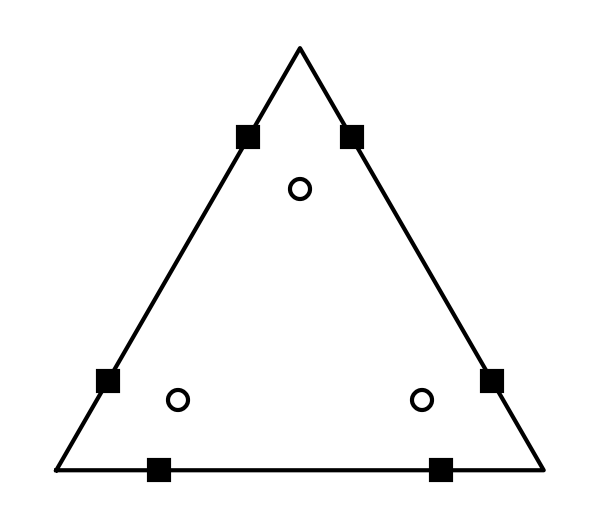
\includegraphics[width=0.16\textwidth]{figures/p1_Omega}\\
                 3 nodes
            \end{center}} &
        \parbox[b]{0.15\textwidth}{%
            \begin{center}%
                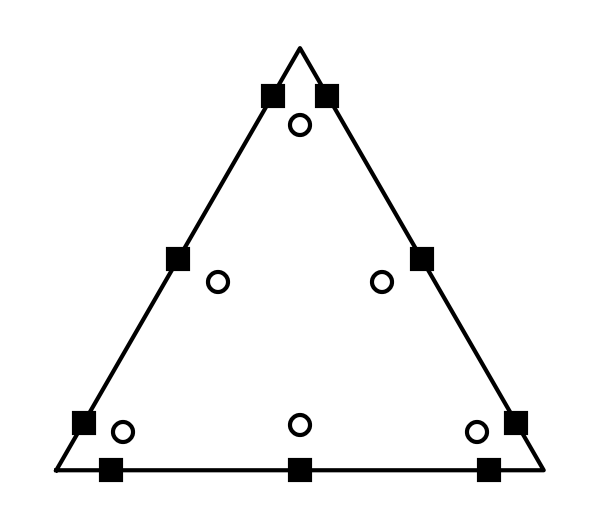
\includegraphics[width=0.16\textwidth]{figures/p2_Omega}\\
                6 nodes
            \end{center}} &
        \parbox[b]{0.15\textwidth}{%
            \begin{center}%
                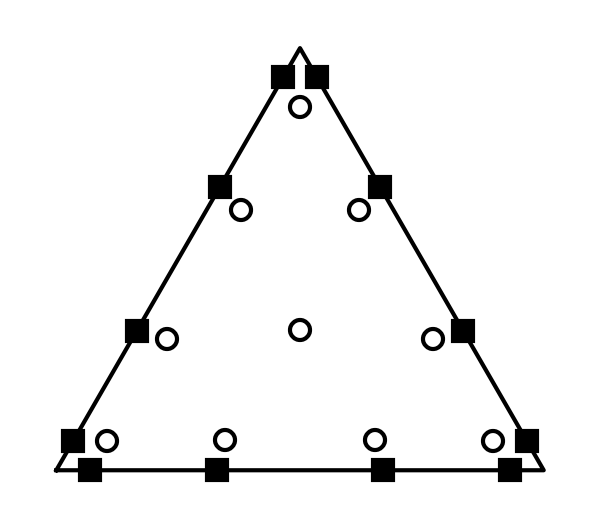
\includegraphics[width=0.16\textwidth]{figures/p3_Omega}\\
                10 nodes
            \end{center}} &
        \parbox[b]{0.15\textwidth}{%
            \begin{center}%
                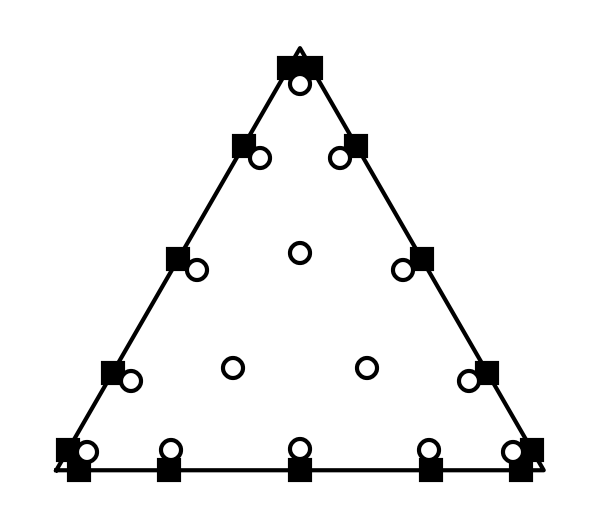
\includegraphics[width=0.16\textwidth]{figures/p4_Omega}\\
                15 nodes
            \end{center}} \\\hline
        \vspace*{-0.15\textwidth}\textbf{SBP}-$\bm{\Gamma}$ & 
        \parbox[b]{0.15\textwidth}{%
            \begin{center}%
                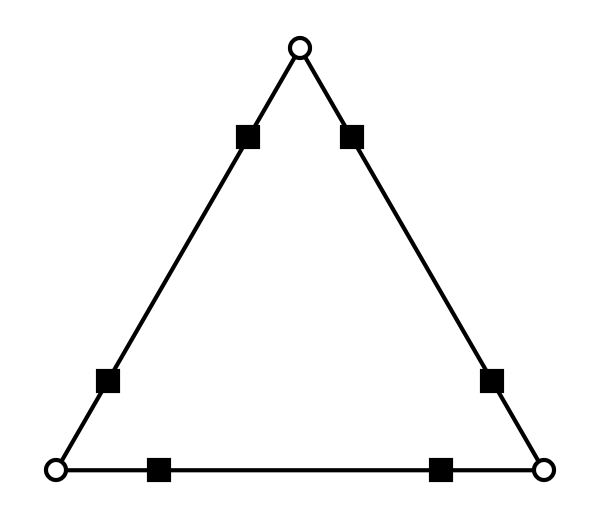
\includegraphics[width=0.16\textwidth]{figures/p1_Gamma}\\
                3 nodes
            \end{center}} &
        \parbox[b]{0.15\textwidth}{%
            \begin{center}%
                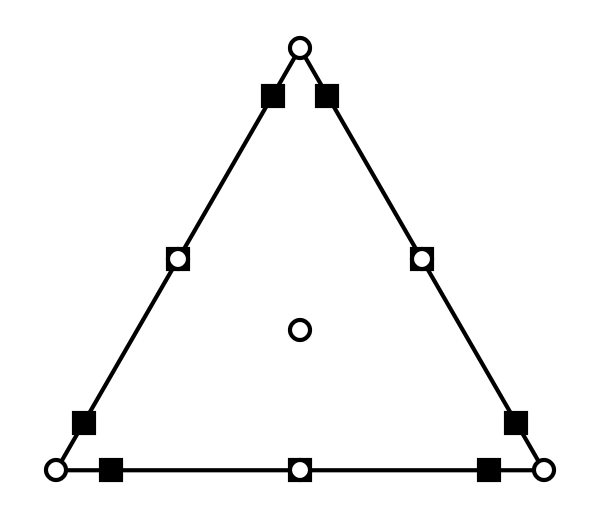
\includegraphics[width=0.16\textwidth]{figures/p2_Gamma}\\
                7 nodes
            \end{center}} &
        \parbox[b]{0.15\textwidth}{%
            \begin{center}%
                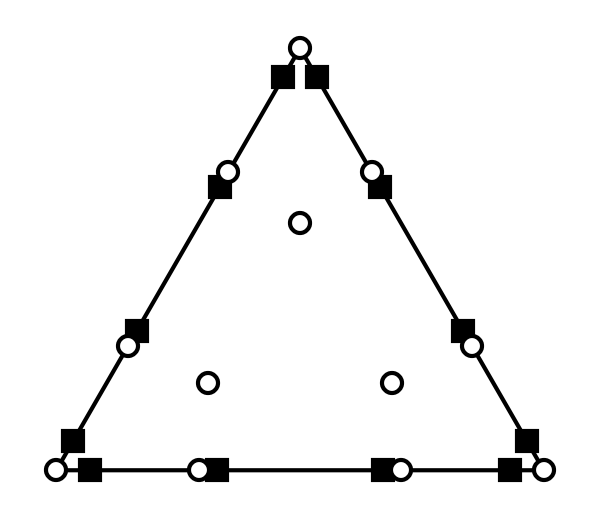
\includegraphics[width=0.16\textwidth]{figures/p3_Gamma}\\
                12 nodes
            \end{center}} &
        \parbox[b]{0.15\textwidth}{%
            \begin{center}%
                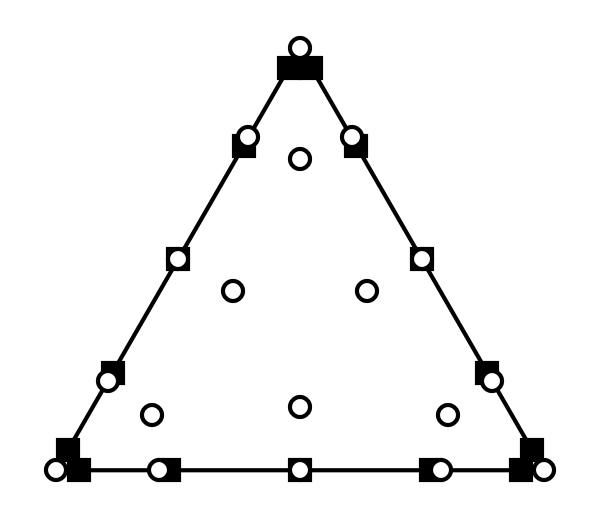
\includegraphics[width=0.16\textwidth]{figures/p4_Gamma}\\
                18 nodes
            \end{center}} \\\hline
    \end{tabular}
\end{frame}

\subsection{Accuracy study}
\begin{frame}{Accuracy study}
    The manufactured solution
    \begin{equation*}
    \begin{aligned}
    \Lambda &= \begin{bmatrix}
    x^2+1 && xy \\ xy && y^2+1
    \end{bmatrix}, \\
    \fnc{U}(x,y) &= \sin(4\pi x)\sin(4\pi y)
    \end{aligned}
    \end{equation*}
   The functional
    \begin{equation*}
    \fnc{J} = \int \fnc{U} \diff \Omega
    \end{equation*}
\end{frame}

\begin{frame}{Accuracy study}
    \vskip -4mm
    \begin{figure}  
        \centering
        \begin{subfigure}[b]{0.425\linewidth}
            \centering
            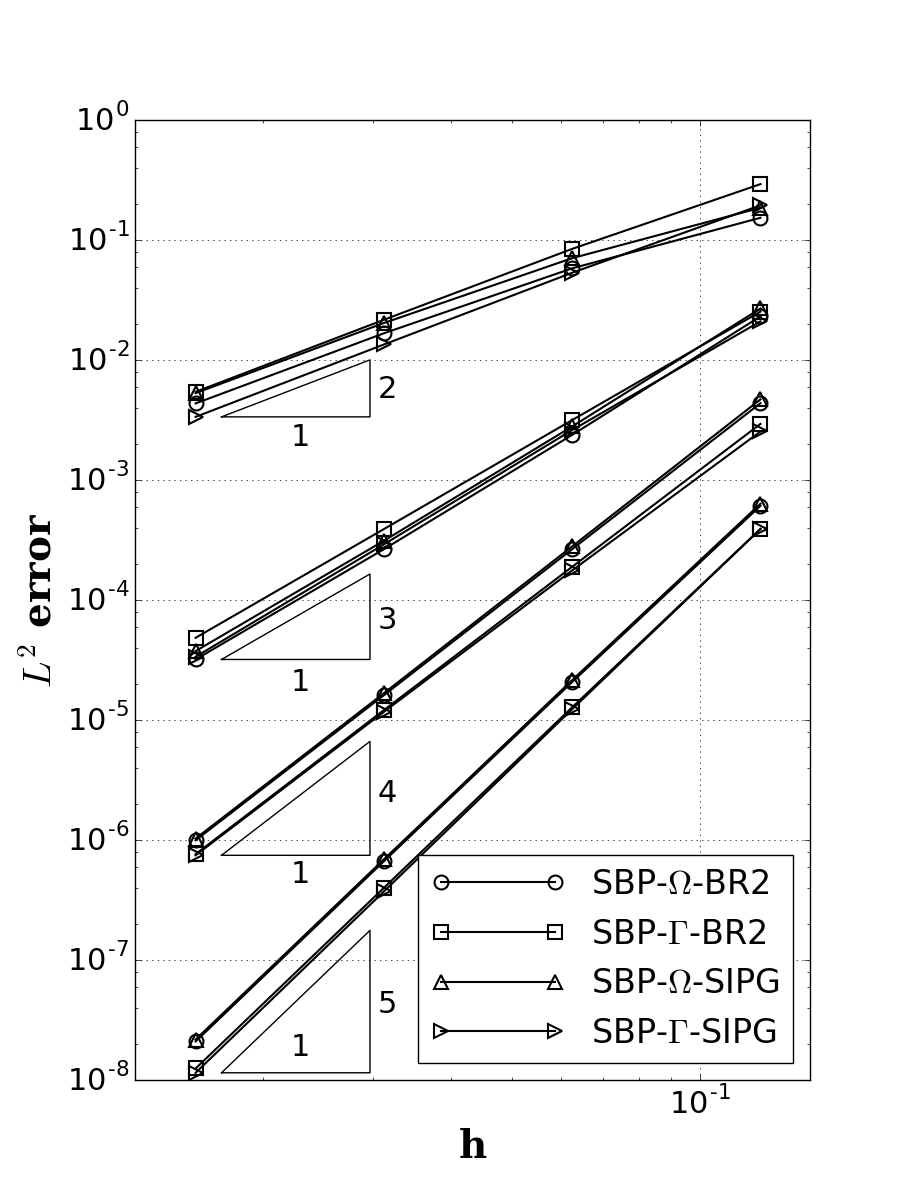
\includegraphics[width=1.0\linewidth]{figures/p_accuracy.png}
            \subcaption*{Error in solution}
        \end{subfigure}%
        \begin{subfigure}[b]{0.425\linewidth}
            \centering
            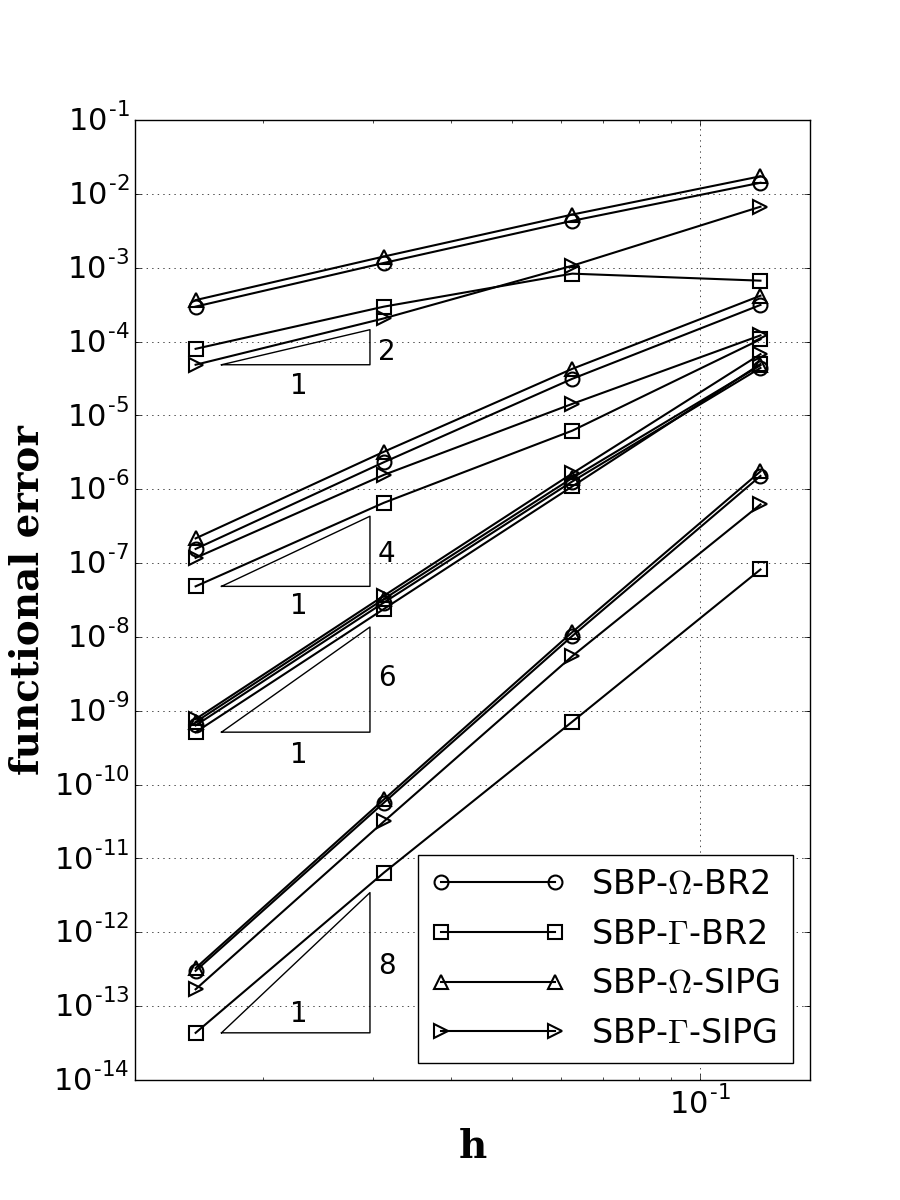
\includegraphics[width=1.0\linewidth]{figures/j_accuracy.png}
            \subcaption*{Error in functional}
        \end{subfigure}
    \end{figure}
\end{frame}

\subsection{Tightness of stability bound}
\begin{frame}{Tightness of stability bound}
    Our stability conditions are sufficient but not necessary, and we want to know how tight they are. To this end, we introduce a relaxation factor 
    $\alpha \in (0,1]$ acting on $\Sig^{(1)}$ and $\Sig^{\fnc{D}}$.
    \begin{itemize}
        \item overly conservative, $\alpha \ll 1$
        \item necessary and sufficient, $\alpha \ge 1$ 
    \end{itemize}
    \begin{figure} 
        \begin{subfigure}{0.45\textwidth}
            \centering
            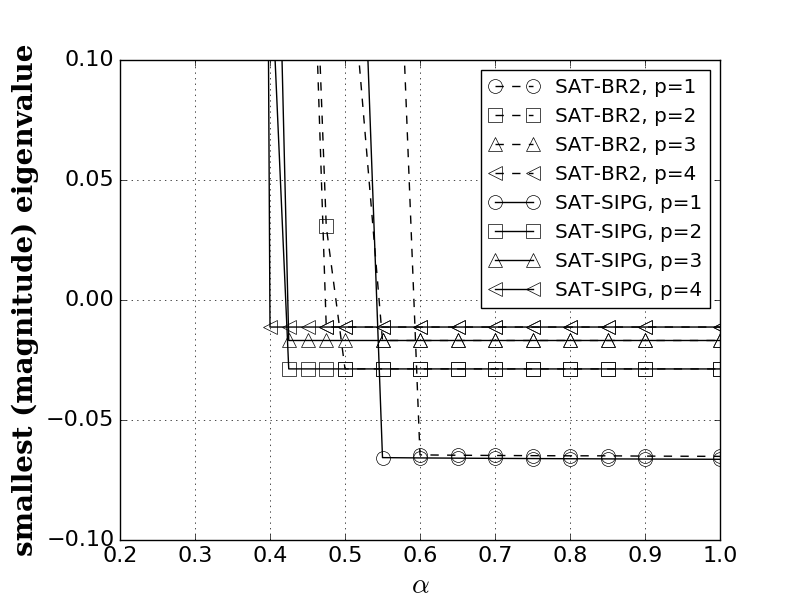
\includegraphics[width=1.0\linewidth]{figures/relaxation_eigMin_gamma.png}
            \subcaption*{\footnotesize Largest eigenvalue using SBP-$\Gamma$}
        \end{subfigure}
        \begin{subfigure}{0.45\textwidth}
            \centering
            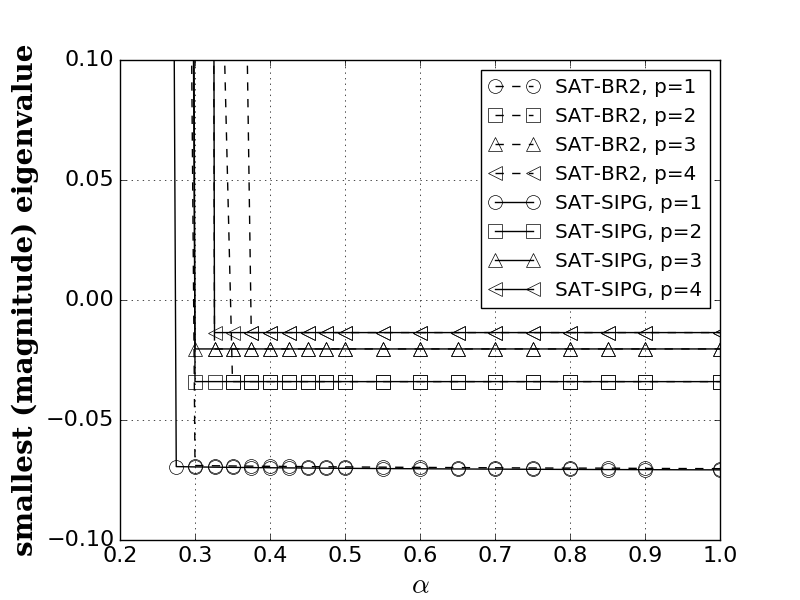
\includegraphics[width=1.0\linewidth]{figures/relaxation_eigMin_omega.png}
            \subcaption*{\footnotesize Largest eigenvalue using SBP-$\Omega$}
        \end{subfigure} 
    \end{figure}

    \begin{textblock}{3.5}(10.5,5.25)
        We solve a steady problem!
    \end{textblock}
\end{frame}

\subsection{Energy stability}

\begin{frame}{Energy stability}
    We solve an unsteady homogeneous problem on a nearly tangled mesh.
    \vskip -2mm
    \begin{figure} 
        \centering
        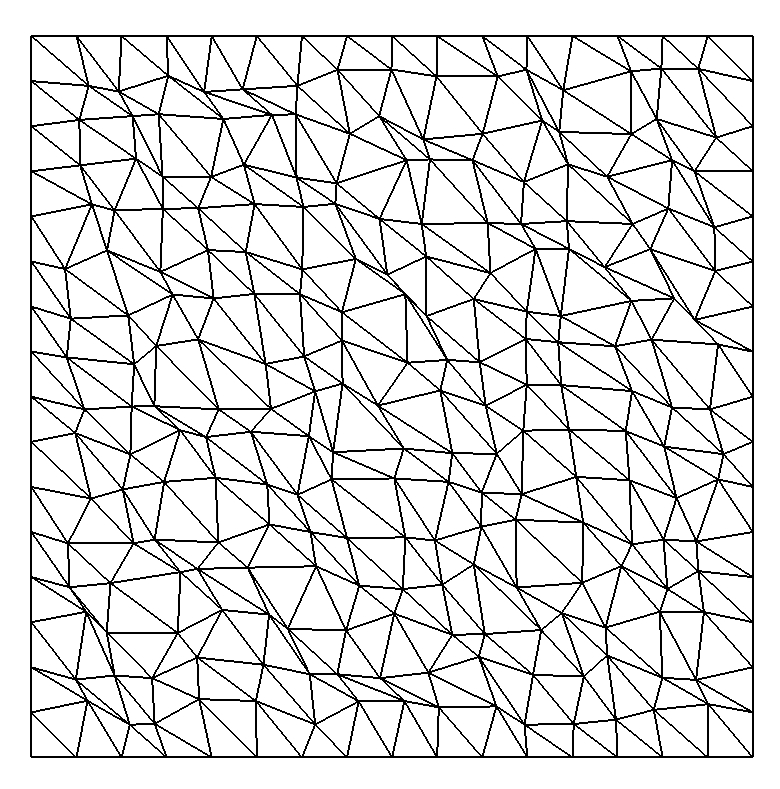
\includegraphics[width=0.45\linewidth]{figures/perturbed_mesh_16x16.png}
        \caption*{\footnotesize Perturbed mesh, the largest angle = 179.90\textdegree}
    \end{figure}
\end{frame}

\begin{frame}{Energy stability}
    We solve an unsteady homogeneous problem on a nearly tangled mesh.
    \vskip -2mm
    \begin{figure} 
        \centering
        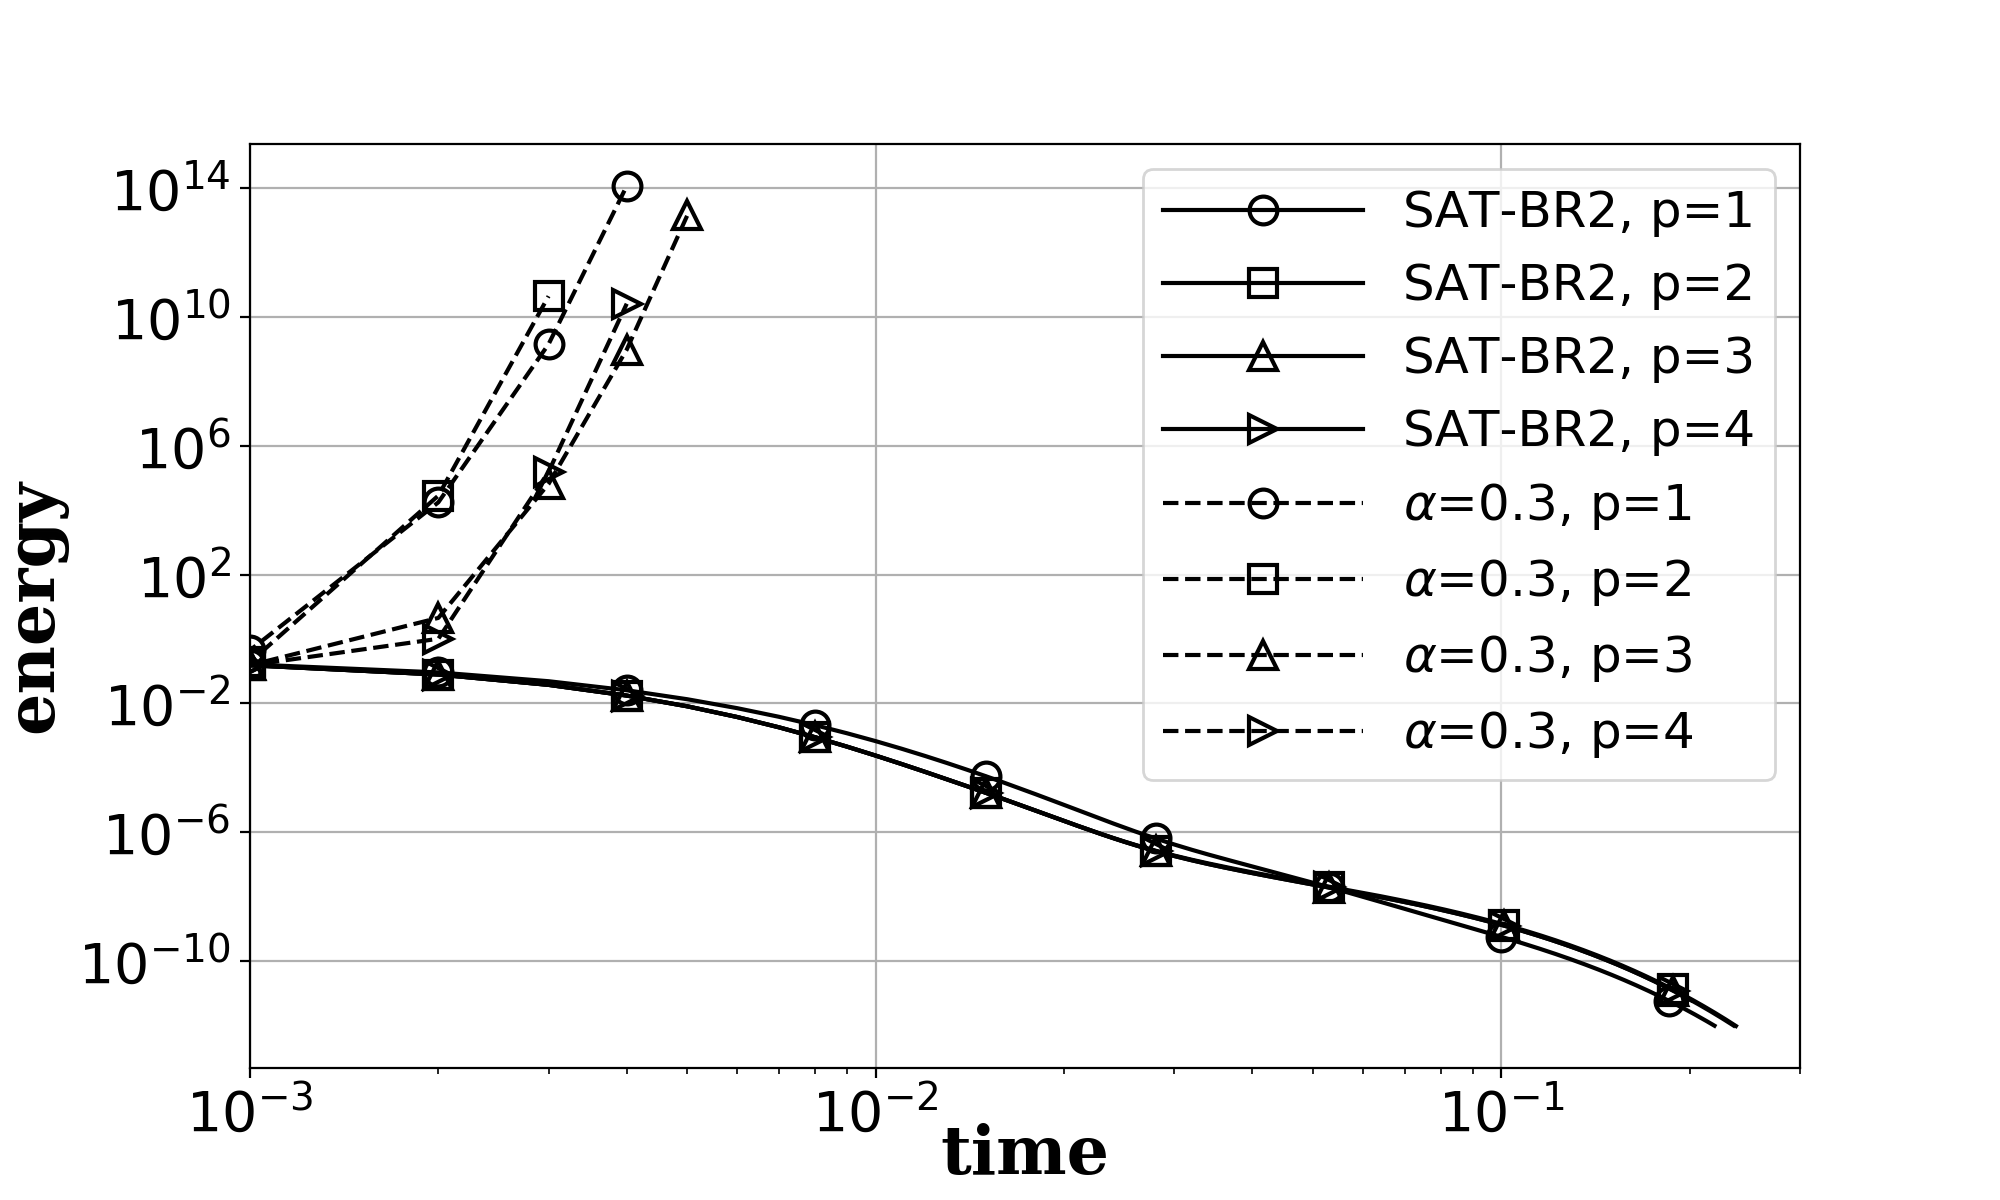
\includegraphics[width=0.75\linewidth]{figures/energy_stability.png}
        \caption*{\footnotesize Energy history of homogeneous problem using BDF2}
    \end{figure}
\end{frame}

\section*{}
\begin{frame}{Conclusion}
      We have
      \begin{itemize}
          \item presented a general discretization with dense penalty matrices;
          \item carried out analysis of adjoint consistency and energy stability, and
          determined conditions that guarantee a conservative, energy-stable,
          primal-consistent, and adjoint-consistent discretization;
          \item generalized BR2 and SIPG, with algebraic connection;
          \item numerically verified the theory.
      \end{itemize}
\end{frame}

\begin{frame}
    \Huge\centering
    Thanks!
\end{frame}

%\begin{frame}[allowframebreaks]{References}
%    \footnotesize
%    \bibliographystyle{plain}
%    \bibliography{references}
%\end{frame}


\end{document}